\documentclass[../thesis.tex]{subfiles}
\graphicspath{{\subfix{../Images/}}}

\begin{document}

\section{Results}
\subsection{Single device}
\begin{figure}[hbt!]
    \begin{subfigure}{.475\linewidth}
            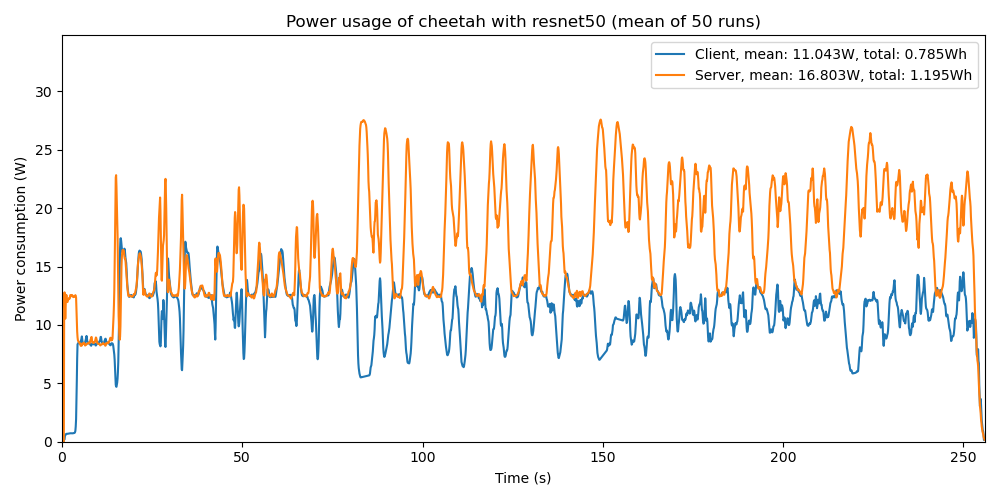
\includegraphics[width=\textwidth]{Thesis/Images/Means/mean_cheetah-resnet50.png}
            \caption{Mean of running Cheetah with resnet50 50 times}
            \label{fig:mean_cheetah_resnet50}
    \end{subfigure}\hfill % <-- "\hfill"
    \begin{subfigure}{.475\linewidth}
            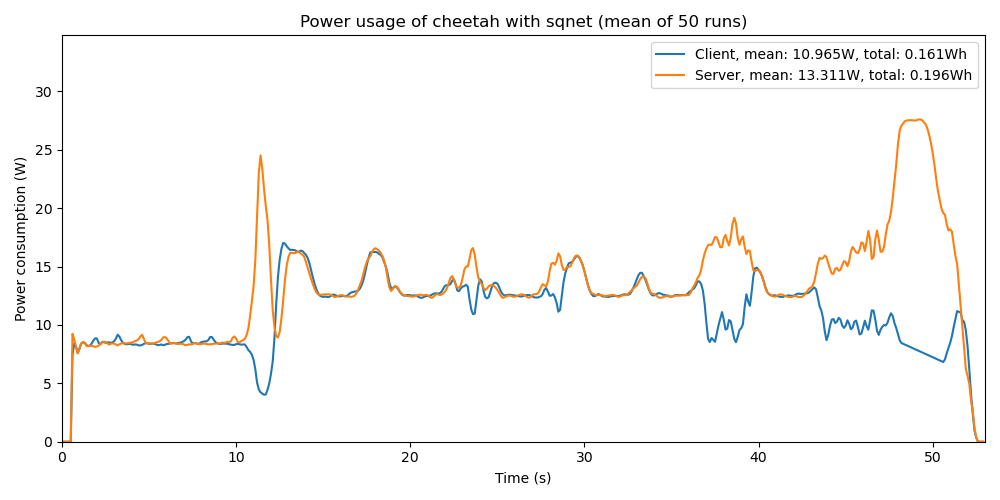
\includegraphics[width=\textwidth]{Thesis/Images/Means/mean_cheetah-sqnet.png}
            \caption{Mean of running Cheetah with sqnet 50 times}
            \label{fig:mean_cheetah_sqnet}
    \end{subfigure}

    \medskip % create some *vertical* separation between the graphs
    
    \begin{subfigure}{.475\linewidth}
            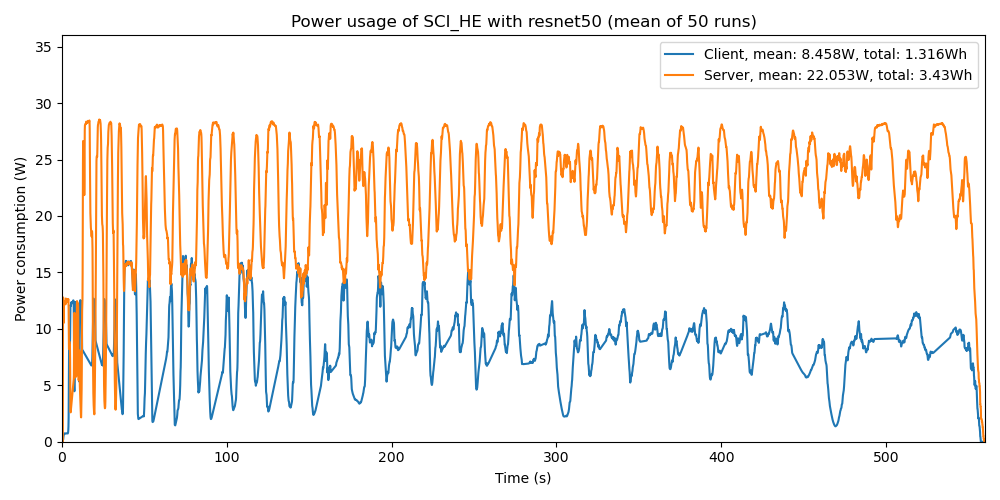
\includegraphics[width=\textwidth]{Thesis/Images/Means/mean_SCI_HE-resnet50.png}
            \caption{Mean of running SCI\_HE with resnet50 50 times}
            \label{fig:mean_SCI_HE_resnet50}
    \end{subfigure}\hfill % <-- "\hfill"
    \begin{subfigure}{.475\linewidth}
            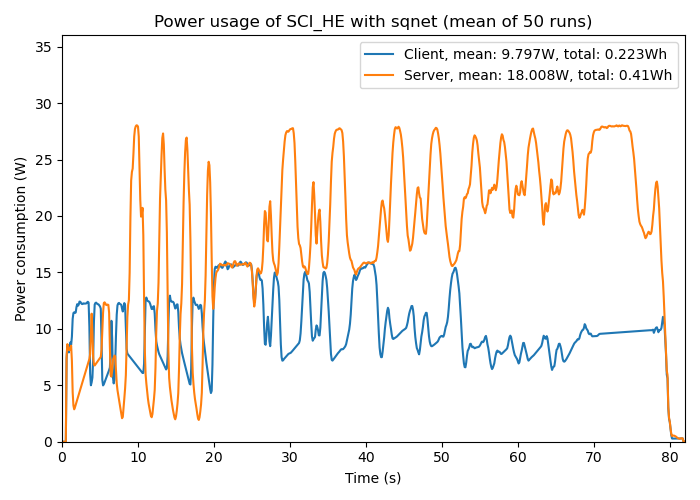
\includegraphics[width=\textwidth]{Thesis/Images/Means/mean_SCI_HE-sqnet.png}
            \caption{Mean of running SCI\_HE with sqnet 50 times}
            \label{fig:mean_SCI_HE_sqnet}
    \end{subfigure}

    \caption{Four measurements doneA figure with four subfigures}
    \label{fig:4results}
\end{figure}
Remarks on Cheetah:
\begin{itemize}
        \item Results Cheetah look very asynchronized, i.e. peaks in power usage on client often mean power throughs. We can see this very good when Cheetah uses the silent OT pack and is synchronising (first 0-10 seconds before the actual inference phase). We can see this best in figure \ref{fig:mean_cheetah_sqnet}. This means that when the server is calculating, the client is running idle.
        \item There are also places in Cheetah where they run syncrhonous. On these places there are peaks for both client and server power usage, e.g. in figure \ref{fig:mean_cheetah_sqnet} between 15-20 seconds. This means that both client and server are calculating.
        \item Idle power consumption with cheetah in the synchronising phase of the silent OT pack is around 9 Watts
        \item Idle power consumption with cheetah in the inference phase is around 12 Watts
        \item With Cheetah the power consumption of server often has peaks when the client has throughs. This is probably because the server is calculating more things than client. This would explain the higher mean of the server side. 
\end{itemize}
Remarks on SCI_HE:
\begin{itemize}
        \item Results $SCI_HE$ also look synchronized. See figure \ref{fig:mean_SCI_HE_sqnet}. This means that either the server or the client is calculating.
        \item I cannot find places where both client and server are calculating. 
        \item While the mean power consumption of the client on $SCI_HE$ is lower then Cheetah, the energy consumption is higher on $SCI_HE$ then Cheetah. This is because the average runtime is higher with $SCI_HE$.
\end{itemize}

% \begin{figure}
%      \centering
%         \begin{subfigure}[b]{0.5\textwidth}
%             \centering
%             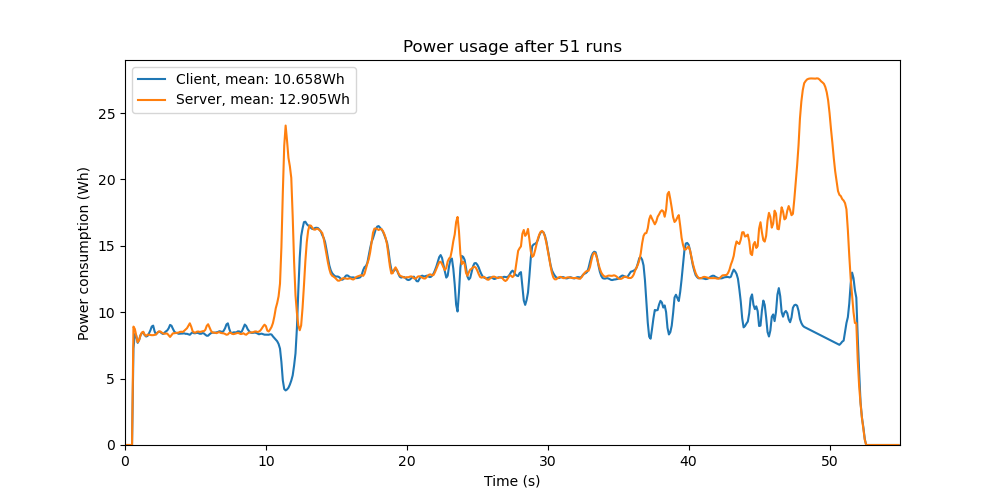
\includegraphics[width=\textwidth]{Thesis/Images/Means/mean_cheetah_resnet50.png}
%             \caption{Mean of running Cheetah with resnet50 51 times}
%             \label{fig:mean_cheetah_resnet50}
%         \end{subfigure}
%         \hfill
%         \begin{subfigure}[b]{0.5\textwidth}
%             \centering
%             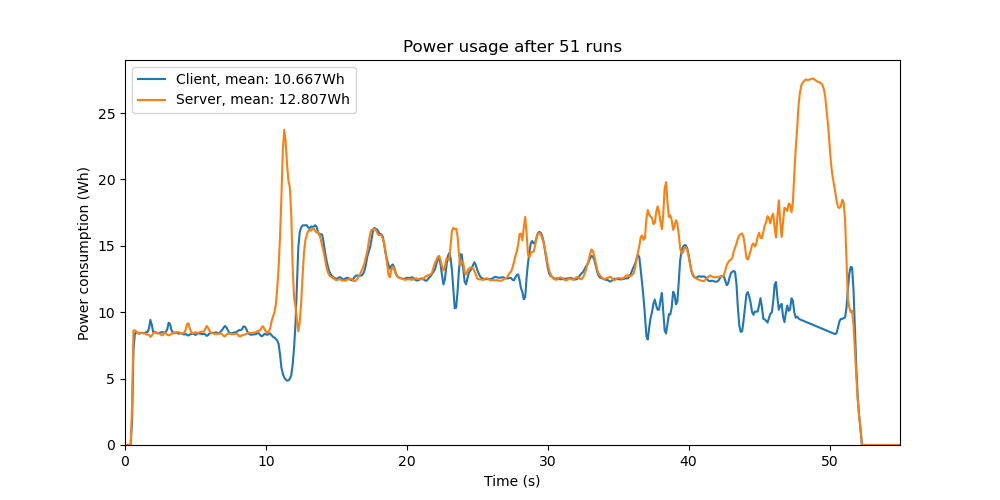
\includegraphics[width=\textwidth]{Thesis/Images/Means/mean_cheetah_sqnet.png}
%             \caption{Mean of running Cheetah with sqnet 51 times}
%             \label{fig:mean_cheetah_sqnet}
%         \end{subfigure}
     
%      \medskip
     
%      \begin{subfigure}
%         \begin{subfigure}[b]{0.5\textwidth}
%             \centering
%             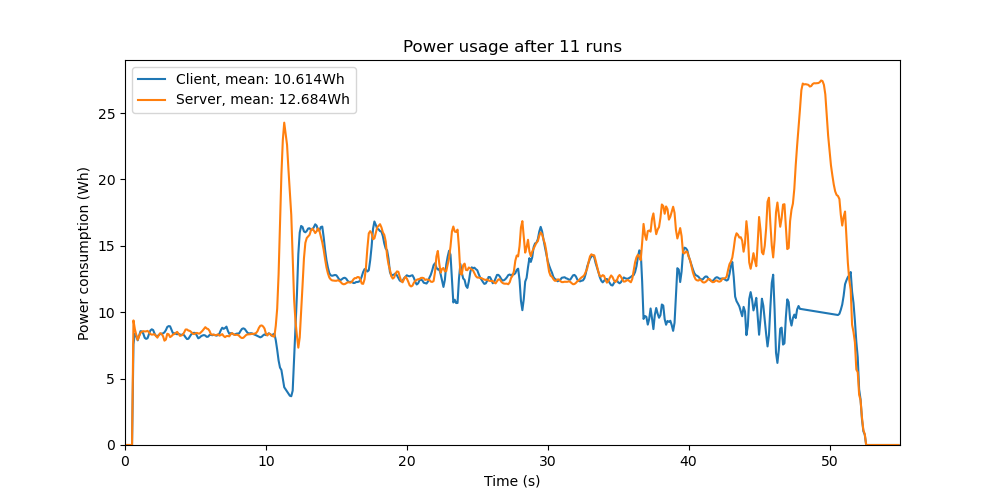
\includegraphics[width=\textwidth]{Thesis/Images/Means/mean_SCI_HE_sqnet.png}
%             \caption{Mean of running SCI_HE with sqnet 11 times}
%             \label{fig:fmean_SCI_HE_sqnet}
%         \end{subfigure}
%         \hfill
%         \begin{subfigure}[b]{0.5\textwidth}
%             \centering
%             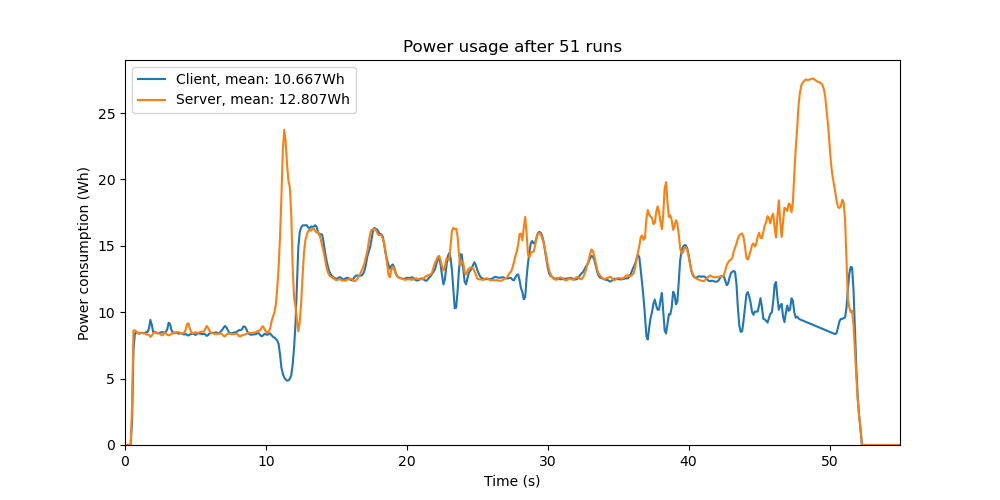
\includegraphics[width=\textwidth]{Thesis/Images/Means/mean_cheetah_sqnet.png}
%             \caption{Mean of running Cheetah with sqnet 51 times}
%             \label{fig:mean_cheetah_sqnet}
%         \end{subfigure}         
%      \end{subfigure}
     
%      \caption{Three simple graphs}
%      \label{fig:three graphs}
% \end{figure}

\subsection{Different devices}
\begin{table}
    \begin{adjustbox}{width=\columnwidth,center}
        \subfile{../Tables/Power_readings_client}
    \end{adjustbox}
    \caption{Power readings of running the Cheetah and $SCI_{HE}$ and limiting the bandwidth of the client.}
    \label{table:powerreadingsclient}
\end{table}

\begin{table}
    \begin{adjustbox}{width=\columnwidth,center}
        \subfile{../Tables/Power_readings_server}
    \end{adjustbox}
    \caption{Power readings of running the Cheetah and $SCI_{HE}$ and limiting the bandwidth of the server.}
    \label{table:powerreadingsserver}
\end{table}

\begin{itemize}
        \item I did not see any increase in energy consumption in the case of Cheetah while changing the server's bandwidth (avg power consumption calculated as sum(Power_i * Runtime_i)/total_i, or sum(Power_client_i * Runtime_client_i + Power_server_i * Runtime_server_i)/Total_i
        \item I did not see any increase in energy consumption in the case of Cheetah while changing the client's bandwidth (with an exception in the case of limiting to 50Mbits => 0.400Wh instead of 3.90Wh)
        \item In the case of CryptFlow2 it is almost the same. Only in the case of limiting to 50Mbits there is a small increase in power consumption
        \item The runtime of CryptFlow2 increased a lot in the case of 50Mbits, but the average power consumption was lower compared to the runs when limiting the bandwidth to higher.
        \item I checked the average data exchanged for both SNNIs without limiting the bandwidth. For cheetah this was around 11/12 Mbits and for CryptFlow this was between 40-60Mbits (high end was on resnet50). This would explain why limiting the bandwidth does not have impact on the power/energy consumption. But if you look at the data exchange between server and client it is sometimes very high and sometimes very low. I thought that because of these data exchange peaks the power/energy consumption would be impacted. One explanation could be that if the data exchange is high, it indeed would take more time, but this also results in a lower power consumption resulting in an energy consumption that is the same. 
\end{itemize}

\begin{table}[]
        \begin{tabular}{ll}
                Generation & Bandwidth \\ \hline
                5G         & 100Mbits  \\ \hline
                LTE        & 30Mbits   \\ \hline
                4G         & 14Mbits   \\ \hline
                3G         & 3Mbits   
        \end{tabular}
        \caption{Average bandwidth of Cellular Broadband Connections}
        \label{table:avg_bandwidth}
\end{table}
Wew can see that limiting the bandwidth has little effect on the energy consumption. This could be explained because the average data exchanged is 11/12Mbits for Cheetah and 40-60Mbits for CryptFlow2. If we look at the average bandwidth of the cellular broadband connections (table \ref{table:avg_bandwidth}) we can see that this would be a problem for Cheetah on 3G. This would also be a problem on 3G and 4G for $SCI_HE$.


\begin{table}
        \begin{adjustbox}{width=\columnwidth,center}
                \subfile{../Tables/Power_readings_client2}
        \end{adjustbox}
        \caption{Power readings of running the Cheetah and $SCI_{HE}$ and limiting the bandwidth of the client.}
        \label{table:powerreadingsclient2}
\end{table}

\begin{table}
        \begin{adjustbox}{width=\columnwidth,center}
                \subfile{../Tables/Power_readings_server2}
        \end{adjustbox}
        \caption{Power readings of running the Cheetah and $SCI_{HE}$ and limiting the bandwidth of the server.}
        \label{table:powerreadingsserver2}
\end{table}
    

I have done the tests, measurements can be found in table \ref{table:powerreadingsclient2} and table \ref{table:powerreadingsserver2}.

\color{red}I still need to do the measurements for limiting both server and client at the same time. This would be a more realistic scenario, since the bottleneck of the route between server and client would be the limiting factor, for both server to client traffic and client to server traffic. I also need to check if limiting the traffic flow would only limit outgoing traffic.\color{black}


\subsection{graphs}
% \begin{figure}[hbt!]
%     \begin{subfigure}{.475\linewidth}
%             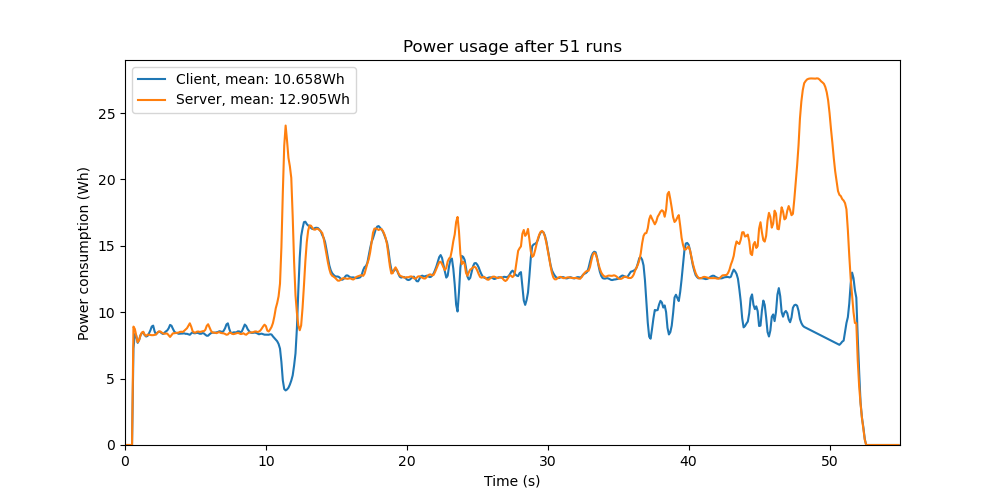
\includegraphics[width=\textwidth]{Thesis/Images/Means/mean_cheetah_resnet50.png}
%             \caption{Mean of running Cheetah with resnet50 51 times}
%             \label{fig:mean_cheetah_resnet50}
%     \end{subfigure}\hfill % <-- "\hfill"
%     \begin{subfigure}{.475\linewidth}
%             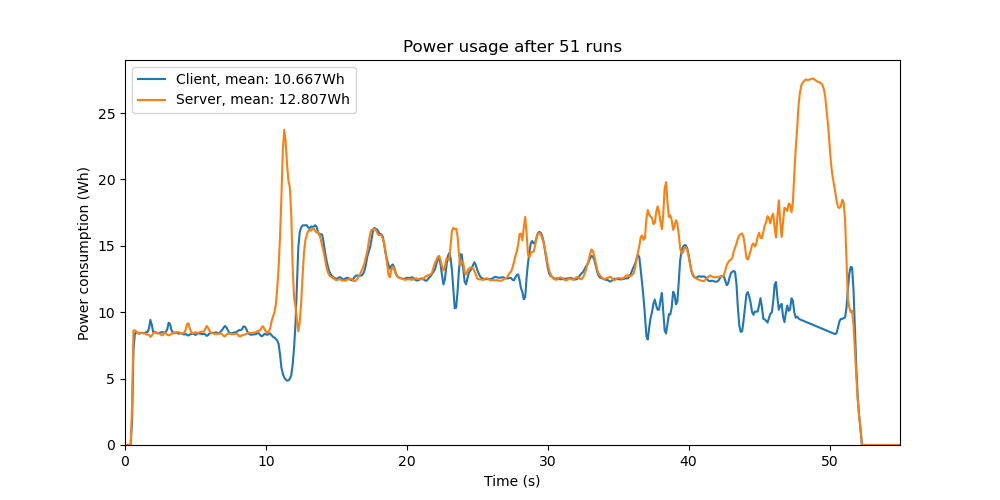
\includegraphics[width=\textwidth]{Thesis/Images/Means/mean_cheetah_sqnet.png}
%             \caption{Mean of running Cheetah with sqnet 51 times}
%             \label{fig:mean_cheetah_sqnet}
%     \end{subfigure}

%     \medskip % create some *vertical* separation between the graphs
    
%     \begin{subfigure}{.475\linewidth}
%             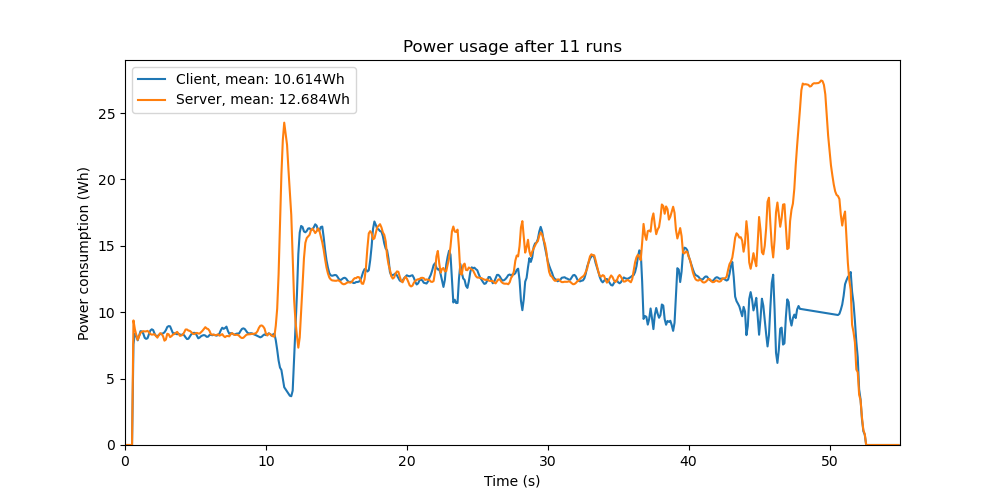
\includegraphics[width=\textwidth]{Thesis/Images/Means/mean_SCI_HE_sqnet.png}
%             \caption{Mean of running SCI\_HE with sqnet 11 times}
%             \label{fig:mean_SCI_HE_sqnet}
%     \end{subfigure}\hfill % <-- "\hfill"
%     \begin{subfigure}{.475\linewidth}
%             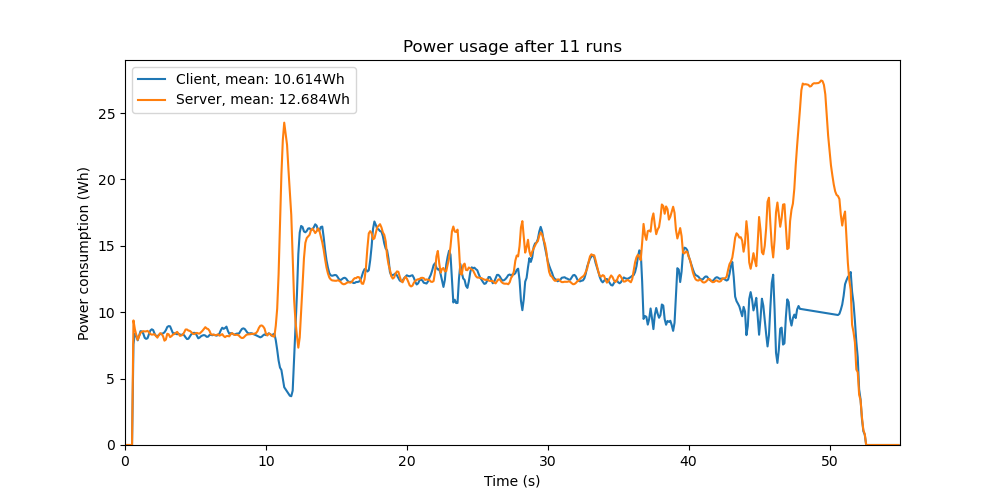
\includegraphics[width=\textwidth]{Thesis/Images/Means/mean_SCI_HE_sqnet.png}
%             \caption{Mean of running SCI\_HE with sqnet 11 times}
%             \label{fig:fmean_SCI_HE_sqnet}
%     \end{subfigure}

%     \caption{Four measurements doneA figure with four subfigures}
%     \label{fig:4results}
% \end{figure}

% \begin{figure}[hbt!]
%     \begin{subfigure}{\linewidth}
%             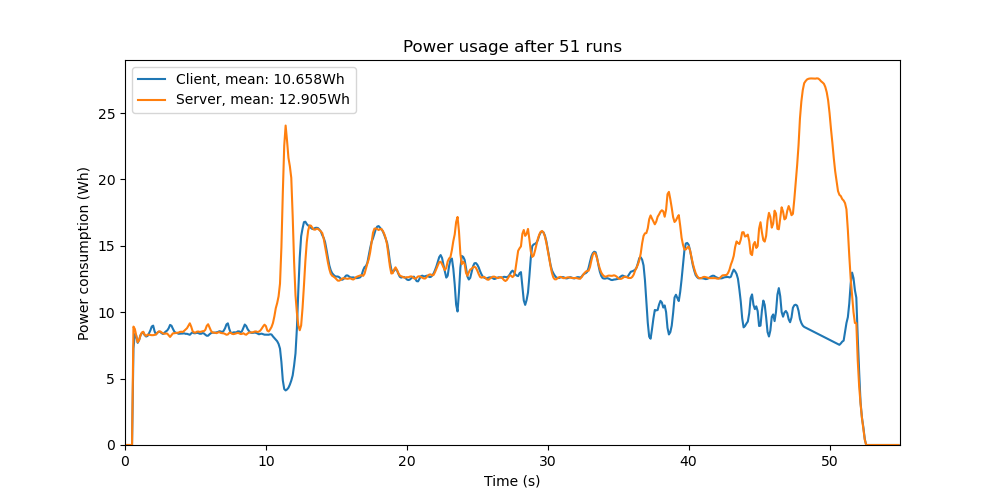
\includegraphics[width=\textwidth]{Thesis/Images/Means/mean_cheetah_resnet50.png}
%             \caption{Mean of running Cheetah with resnet50 51 times}
%             \label{fig:bmean_cheetah_resnet50}
%     \end{subfigure}
%     \begin{subfigure}{\linewidth}
%             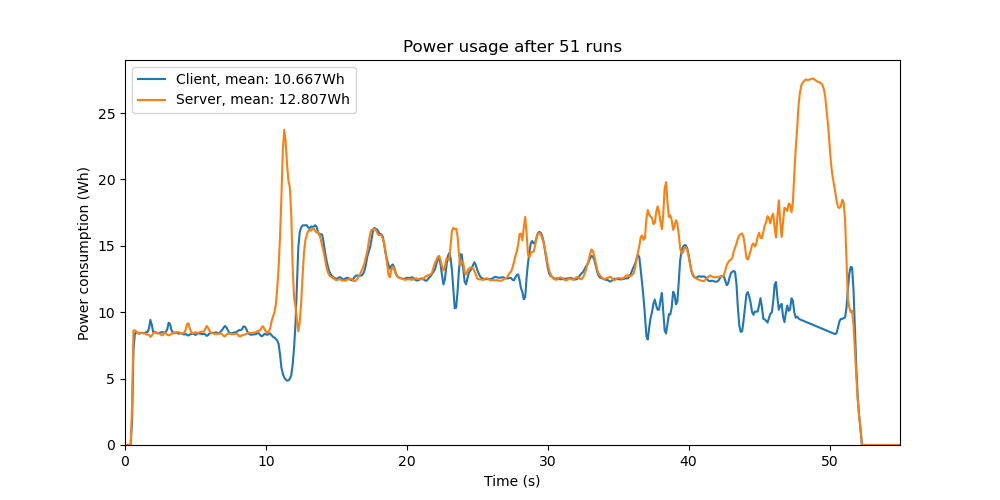
\includegraphics[width=\textwidth]{Thesis/Images/Means/mean_cheetah_sqnet.png}
%             \caption{Mean of running Cheetah with sqnet 51 times}
%             \label{fig:bmean_cheetah_sqnet}
%     \end{subfigure}    
%     \begin{subfigure}{\linewidth}
%             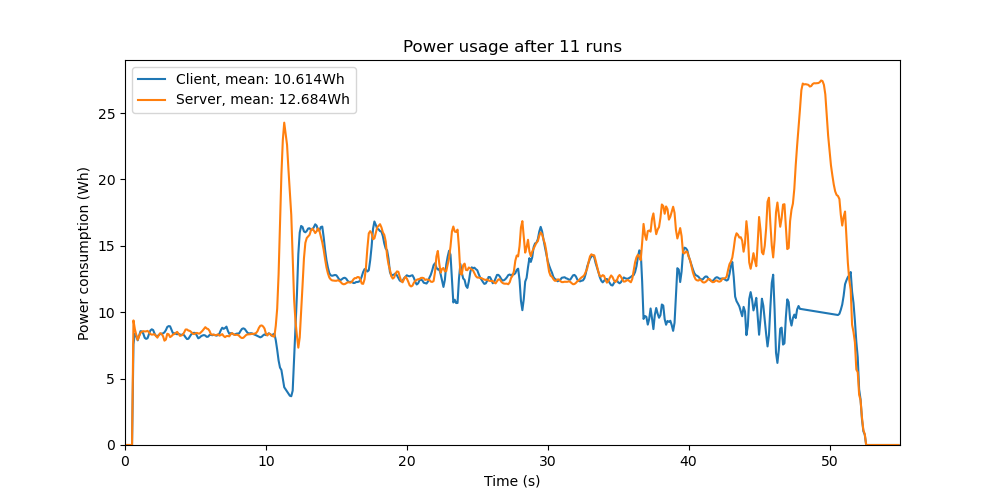
\includegraphics[width=\textwidth]{Thesis/Images/Means/mean_SCI_HE_sqnet.png}
%             \caption{Mean of running SCI\_HE with sqnet 11 times}
%             \label{fig:bmean_SCI_HE_sqnet}
%     \end{subfigure}
%     \begin{subfigure}{\linewidth}
%             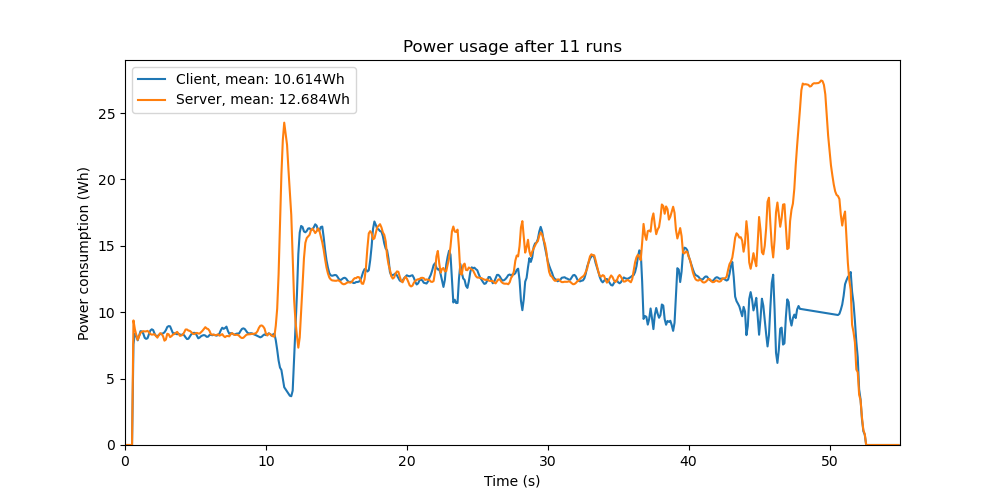
\includegraphics[width=\textwidth]{Thesis/Images/Means/mean_SCI_HE_sqnet.png}
%             \caption{Mean of running SCI\_HE with sqnet 11 times}
%             \label{fig:bfmean_SCI_HE_sqnet}
%     \end{subfigure}

%     \caption{Four measurements doneA figure with four subfigures}
%     \label{fig:4results2}
% \end{figure}

\noindent
% Cross-references to subfigures \ref{fig:mean_cheetah_resnet50}, \ref{fig:mean_cheetah_sqnet} and \ref{fig:mean_SCI_HE_sqnet} and of figure \ref{fig:4results}.

% \begin{figure}[h!]
%     \centering
%     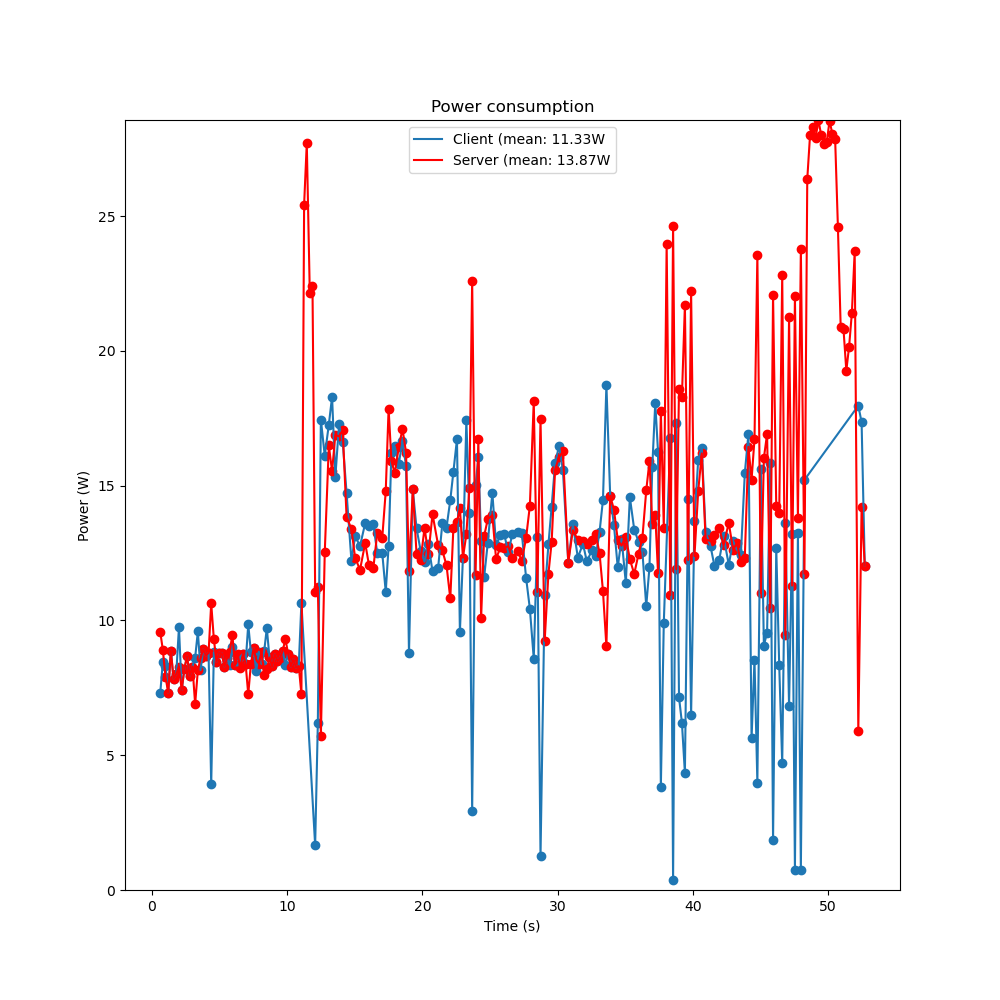
\includegraphics[width=\textwidth,height=\textheight,keepaspectratio]{cheetah-sqnet.png}
%     \caption{Running the SNNI cheetah on sqnet}
%     \label{fig:my_label}
% \end{figure}
% \newpage
% \begin{figure}[h!]
%     \centering
%     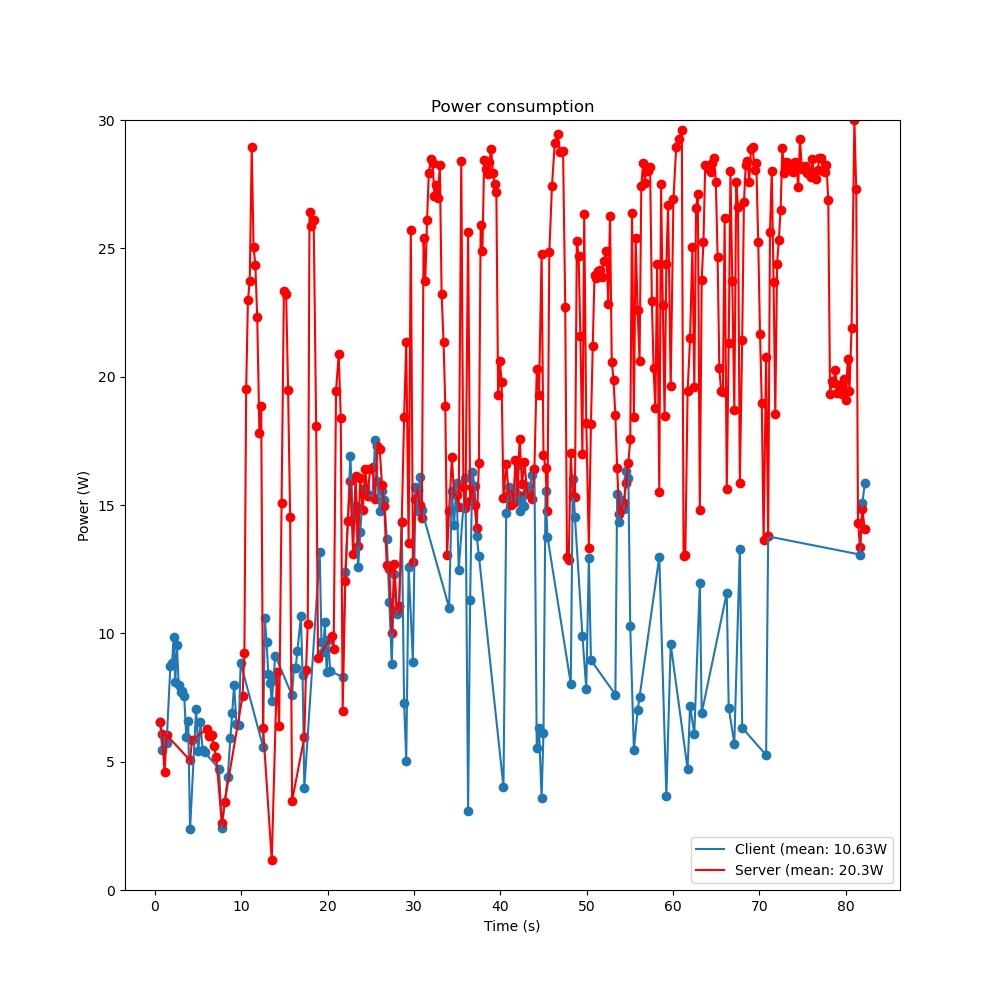
\includegraphics[width=\textwidth,height=\textheight,keepaspectratio]{SCI_HE-sqnet.png}
%     \caption{Running the SNNI CryptFlow2 on sqnet}
%     \label{fig:my_label}
% \end{figure}
\section{RQb, what are the differences on server and client side and what are the implications}
\end{document}
